\documentclass[a4paper]{article}
\usepackage[utf8x]{inputenc}
\usepackage[T1,T2A]{fontenc}
\usepackage[russian]{babel}
\usepackage{hyperref}
\usepackage{indentfirst}
\usepackage{listings}
\usepackage{color}
\usepackage{here}
\usepackage{array}
\usepackage{multirow}
\usepackage{graphicx}

\usepackage{caption}
\renewcommand{\lstlistingname}{Программа} % заголовок листингов кода

\usepackage{listings}
\lstset{ %
extendedchars=\true,
keepspaces=true,
language=bash,					% choose the language of the code
basicstyle=\footnotesize,		% the size of the fonts that are used for the code
numbers=left,					% where to put the line-numbers
numberstyle=\footnotesize,		% the size of the fonts that are used for the line-numbers
stepnumber=1,					% the step between two line-numbers. If it is 1 each line will be numbered
numbersep=5pt,					% how far the line-numbers are from the code
backgroundcolor=\color{white},	% choose the background color. You must add \usepackage{color}
showspaces=false				% show spaces adding particular underscores
showstringspaces=false,			% underline spaces within strings
showtabs=false,					% show tabs within strings adding particular underscores
frame=single,           		% adds a frame around the code
tabsize=2,						% sets default tabsize to 2 spaces
captionpos=b,					% sets the caption-position to bottom
breaklines=true,				% sets automatic line breaking
breakatwhitespace=false,		% sets if automatic breaks should only happen at whitespace
escapeinside={\%*}{*)},			% if you want to add a comment within your code
postbreak=\raisebox{0ex}[0ex][0ex]{\ensuremath{\color{red}\hookrightarrow\space}}
}

\usepackage[left=2cm,right=2cm,
top=2cm,bottom=2cm,bindingoffset=0cm]{geometry}


\begin{document}	% начало документа

\begin{titlepage}	% начало титульной страницы

	\begin{center}		% выравнивание по центру

		\large Санкт-Петербургский Политехнический Университет Петра Великого\\
		\large Институт компьютерных наук и технологий \\
		\large Кафедра компьютерных систем и программных технологий\\[6cm]
		% название института, затем отступ 6см
		
		\huge Программирование\\[0.5cm] % название работы, затем отступ 0,5см
		\large Отчет по выполнению проекта\\[0.1cm]
		\large Японская игра Сёги\\[5cm]

	\end{center}


	\begin{flushright} % выравнивание по правому краю
		\begin{minipage}{0.25\textwidth} % врезка в половину ширины текста
			\begin{flushleft} % выровнять её содержимое по левому краю

				\large\textbf{Работу выполнил:}\\
				\large Леженин Ю.И.\\
				\large {Группа:} 13501/4\\
				
				\large \textbf{Преподаватель:}\\
				\large Вылегжанина К.Д.

			\end{flushleft}
		\end{minipage}
	\end{flushright}
	
	\vfill % заполнить всё доступное ниже пространство

	\begin{center}
	\large Санкт-Петербург\\
	\large \the\year % вывести дату
	\end{center} % закончить выравнивание по центру

\thispagestyle{empty} % не нумеровать страницу
\end{titlepage} % конец титульной страницы

\vfill % заполнить всё доступное ниже пространство



% Содержание
\tableofcontents
\newpage



\section{Японская игра Сеги}

\subsection{Игровые принадлежности}

Доска сёги – 9x9 клеток, нумерующихся сверху вниз и справа налево. Клетки имеют прямоугольную форму, никак не обозначены и не имеют цвета. «Сверху» расставляются в три ряда белые фигуры – пятиугольные дощечки с обозначениями фигур. Играют два игрока. «Белые» и «черные» – это обозначение играющих, фигуры в сёги одного цвета, принадлежность последних определяется направлением острого угла дощечки. Фигура всегда устанавливается острой стороной к противнику. У каждого игрока по 20 фигур 8 наименований, отличающихся друг от друга своей ценностью, силой и рисунком ходов.

У каждой стороны есть один король, одна ладья, один слон, два золотых генерала, два серебряных генерала, два коня, два копья и девять пешек. В крайнем ряду, рядом с копьями располагаются кони. Рядом с конями – серебряные генералы. Рядом с серебряными генералами – золотые генералы. В центре, между двумя золотыми генералами находится король. На втором ряду – только две фигуры. Перед конем с левой стороны находится слон. Перед конем с правой стороны – ладья. В третьем ряду расположены девять пешек.

\subsection{Порядок игры}

Игроки делают ходы поочередно. Первые ходят чёрные. Ход представляет собой перемещение одной из фигур своего цвета, имеющихся на доске, на любое разрешенное поле согласно правилам передвижения фигур или выставление (сброс) фигуры находящейся в резерве. Фигуры «в резерве» (или по-другому «в руке») – это фигуры, взятые (сбитые) у противника.

В сёги при достижении фигурами специальной зоны (лагерь противника) они могут быть усилены (превращены). При превращении фигура переворачивается. В сёги усилиться может любая фигура кроме короля и золотого генерала.

Цель игры – поставить мат королю противника. Считается, что поставлен мат, когда король находится под ударом вражеской фигуры, т.е. находится в поле, куда может походить вражеская фигура, а возможности защититься или уйти нет.

\subsection{Взятие фигур}

«Взятие» – это ход на поле, занятое фигурой противника. В этом случае фигура противника снимается с доски и размещается рядом с ней. В отличие от шахмат, где взятые фигуры удаляются до конца игры, в сёги они могут в дальнейшем быть использованы как свои. Эти фигуры находятся в «резерве» («в руке») и в любой момент такая фигура может быть выставлена (сброшена) на любое свободное поле. 

\subsection{Ходы фигур}

\begin{itemize}
	\item Король, 
	 ходит как шахматный король — на одно поле в любом направлении.
	 
	\item Ладья, ходит как шахматная ладья — на любое количество полей по горизонтали и 	     вертикали.

	 После превращения:

     Дракон, ходит и как ладья, и как король.

	\item Слон,ходит как шахматный слон — на любое число полей по диагонали.

	 После превращения:

	 Лошадь, ходит и как слон, и как король.

	\item Золотой генерал, ходит на любое соседнее поле, кроме полей сзади по диагонали.

	\item Серебряный генерал, ходит на любое соседнее поле, кроме полей справа, слева и 	 	 снизу.

	 После превращения:

	 Перевёрнутый серебряный генера, ходит как золотой генерал.

	\item Конь, ходит буквой «Т» вперёд, то есть на два поля вперёд, и сразу на одно поле 		 вправо или влево. Единственная фигура сёги, которая может перескакивать через другие 		 фигуры.

	 После превращения:

     Перевёрнутый конь, ходит как золото.

	\item Копьё, ходит на любое число полей прямо вперёд. Иногда, также, называется стрела 	 или пика.

	 После переворота:

	 Перевёрнутое копьё, Ходит как золото.

    \item Пешка, ходит на одно поле прямо вперёд. Бьёт так же, как и ходит.

	 После переворота:

	 Перевёрнутая пешка, ходит как золото.
	
\end{itemize}

\subsection{Превращение}

Когда фигура достигает лагеря противника (зоны превращения) у неё возникает возможность стать превращенной (исключение составляют лишь король и золотой генерал, которые превращаться не могут). Но превращение не является обязательным, оно может быть осуществлено при любом очередном ходе (сначала передвижение, затем превращение), но только если эта фигура по-прежнему находится в лагере противника. Фигура может быть также превращена за пределами зоны превращения – в момент выхода из нее. При превращении фигура переворачивается сразу после хода и приобретает свойства превращенной фигуры. Для большинства фигур это способности золотого генерала, ладья и слон превращаются соответственно в короля-дракона и коня-дракона. Обратное превращение не допускается.

Превращение обязательно для фигур, которые не могут продолжать игру со свойствами непревращенных фигур, такие случаи возможны для пешки, копья и коня.

Если превращенная фигура взята противником, то она теряет свои способности и приобретает первоначальные свойства. Выставление

Фигура, находящаяся «в руке», может быть выставлена (сброшена) на любое свободное поле доски, что считается очередным ходом. Фигура сбрасывается только в непревращённом виде (даже если она была превращенной до взятия). Нельзя выставляться на поле занятое фигурой противника. После выставления фигура приобретает те же права, что и находящиеся на доске. Если фигура сброшена в лагерь противника, она может превратиться, только сделав следующий ход, даже если он сделан на поле за пределами зоны превращения.

\subsection{Запрещенные ходы}

Следующие ходы запрещены:

\begin{itemize}

	\item Сдваивание пешек (нифу). Когда на одной из вертикалей имеется не превращённая 		 пешка, не разрешается выставлять другую пешку на ту же вертикаль.
	
	\item Выставление пешки с матом (учи-фу-тсумэ). Не разрешается выставлять пешку с 			 матом королю противника. Однако объявлять мат очередным ходом пешки, находящейся на 		 доске, разрешено.
	
	\item Выставленние фигуры запертой. Запрещается сбрасывать фигуры таким образом, что у 	 них будет отсутствовать возможность хода в дальнейшем.
	
\end{itemize}

Игроку, сделавшему запрещенный ход, может быть присуждено поражение.

\subsection{Ничья}

Большинство партий в сёги оканчиваются либо матом, либо признанием поражения одним из игроков, однако ничья также возможна.

\begin{itemize}


	\item Повторение
	
	Пытаясь избежать проигрыша или ухудшения позиции, возможные как для одной, так и для 		другой стороны, игроки могут сознательно повторять ходы. Ничья объявляется при 				четырёхкратном повторении ситуации на доске с учетом захваченных фигур.


	\item Вечный шах

	В сёги нельзя форсировать ничью вечным шахом, как в шахматах. Если в результате серии 		шахов одного из соперников, позиция была повторена троекратно, то шахующий обязан 			изменить свой ход, иначе ему будет засчитано поражение.
   
\end{itemize}


\section{Проектирование}

\subsection{Концепция приложения} 

Созданное приложение должно предполагать возможность игры двух игроков (человека и человека или человека и компьютера). Кроме того, необходимо реализовать систему сохранения и загрузки игровых партий. Также, приложение должно обладать графическим интерфейсом, позволяющим выполнять вышеперечисленные действия.

\subsection{Минимально работоспособный продукт}

Консольное приложение, позволяющие вести игру в Сёги двум игрокам.

\subsection{Прецеденты использования}

На основе разработанной концепции была составлена UML диаграмма прцедентов использования.

\begin{figure}[H]
	\begin{center}
		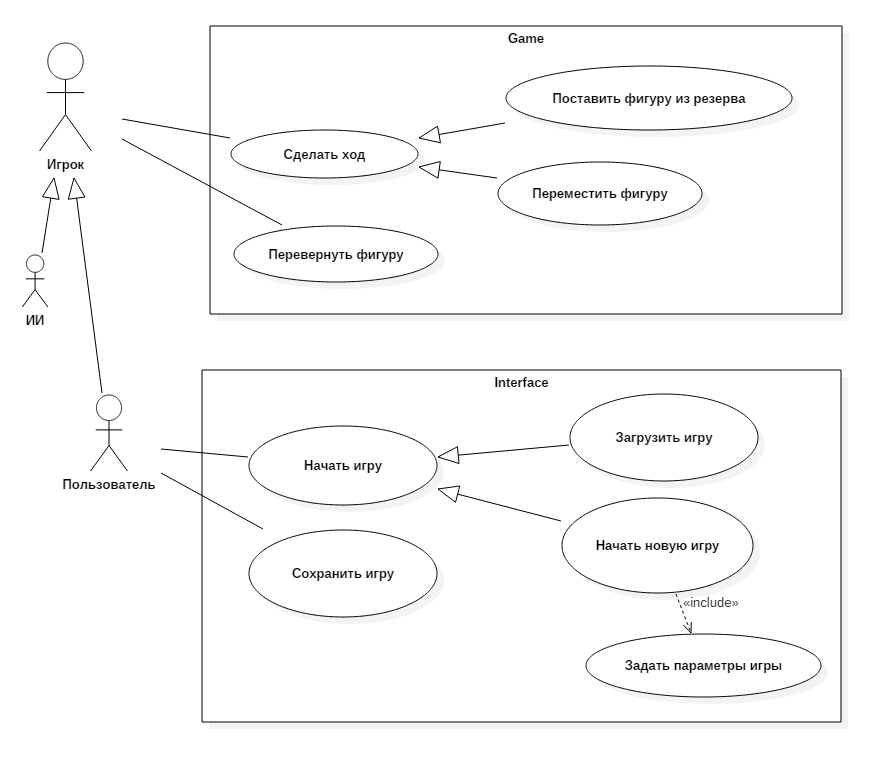
\includegraphics[scale=0.5]{../diagrams/UseCaseDiagram1.png}
		\caption{Диаграмма прцедентов использования}
		\label{pic:use_case}
	\end{center}
\end{figure}

Прецеденты были разделены на 2 части. Первая часть относиться к игровой логике, а вторая к интерфейсу приложения, взаимодействующему с пользователем.

\subsection{Компоненты}

На основе анализа концепции и выделенных прецедентов использования было принято решение выделить три компонента, которые будут входить в состав продукта: библиотека, содержащая игровую модель и механику игры, консольное и графическое приложения.

\begin{figure}[H]
	\begin{center}
		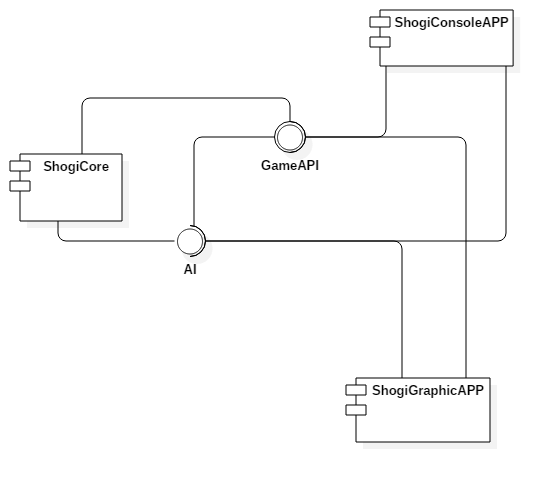
\includegraphics[scale=0.7]{../diagrams/ComponentDiagram1.png}
		\caption{Диаграмма компонентов}
		\label{pic:components}
	\end{center}
\end{figure}

\subsubsection{Библиотека}

\subsubsection{Консольное приложение}

\subsubsection{Графическое приложение}

\subsection{Структура генерируемых файлов}

В ходе работы приложение предполагается создавать файлы сохранения, открывать и читать их. Для того, чтобы обеспечить удобный парсинг файлов сохранения было решено использовать формат JSON. Этот формат легко читается как компьютером, так и человеком. Кроме того, существует множество готовых инструментов предназначенных для работы с JSON, которые могли бы использоваться в процессе разработки.

\captionof{lstlisting}{save\_example.json} 
\lstinputlisting[label=code:hello]{../save_example.json}

Файл сохранения содержит информацию об очередности хода, список фигур на доске и их положение, спиок захваченных фигур.

\subsection{Инструменты}

\section{Реализация}


\section{Процесс обеспечения качества и тестирование}


\section{Выводы}


\section{Приложение 1}

\section{Приложение 2}

%\subsection{Листинг}
%
%\captionof{lstlisting}{hell\_o.c} % для печати символ '_' требует выходной символ '\'
%\lstinputlisting[label=code:hello]{listings/hell_o.c}
%\parindent=1cm % командна \lstinputlisting сбивает параментры отступа
%Текст без отступа (следует за вставкой)
%
%Новый параграф
%
%\noindent Новый параграф с принудительно выключенным отступом
%
%
%\subsection{Частичный листинг}
%% настрока частичного ввода (требуется один раз)
%\makeatletter
%\def\lst@PlaceNumber{\llap{\normalfont
%                \lst@numberstyle{\the\lst@lineno}\kern\lst@numbersep}}
%\makeatother
%
%\captionof{lstlisting}{фрагмент hell\_o.c}
%\lstinputlisting[label=code:hello_mod, linerange={4-5}]{listings/hell_o.c}
%\parindent=1cm
%
%\subsection{Таблица}
%
%\begin{table}[H]
%	\begin{center}
%		\begin{tabular}{|l|l|}
%			\hline
%			top left & top right\\ \hline
%			bot left & bot right\\ \hline
%		\end{tabular}
%		\caption{ Название таблицы}
%		\label{tabular:tab_examp}
%	\end{center}
%\end{table}
%
\end{document}